\documentclass[en,navbaroff]{sdqbeamer} %compiles with lualatex
\titleimage{banner}
\groupname{IPE}
\grouplogo{IPElogo} %add additional logo in the cls file
\title[Master Thesis]{A Terabit-Sampling System with a Photonics Time-Stretch ADC}
\subtitle{Master Thesis Presentation} 
\author[Olena Manzhura]{Olena Manzhura}
\date[\today]{\today}

%Literatur 
\usepackage[citestyle=authoryear,bibstyle=numeric,hyperref,backend=biber]{biblatex}
\addbibresource{lit.bib}
\bibhang1em

\usepackage{amssymb}
\usepackage{amsmath}
\usepackage{mathtools}
\usepackage{booktabs}
\usepackage{siunitx}
\usepackage{graphicx}
\sisetup{range-phrase=...}
\usepackage{tikz}
\usetikzlibrary{external}
\tikzexternalize[optimize=false,prefix=tikz/]
\usepackage{tikzscale}
\usepackage{pgfgantt}
\usepackage{soul}
\usepackage{pgfplots}
\pgfplotsset{compat=newest}
\usepackage{tikzscale}
\usepackage[european]{circuitikz}
\usepackage{animate}
\usepgfplotslibrary{fillbetween}
\usepgfplotslibrary{groupplots}



\begin{document}
\KITtitleframe
\begin{frame}[t]{Agenda}
\tableofcontents[hideallsubsections]
\end{frame}

\section{Introduction}
\begin{frame}[t]{Introduction}
	\begin{figure}
		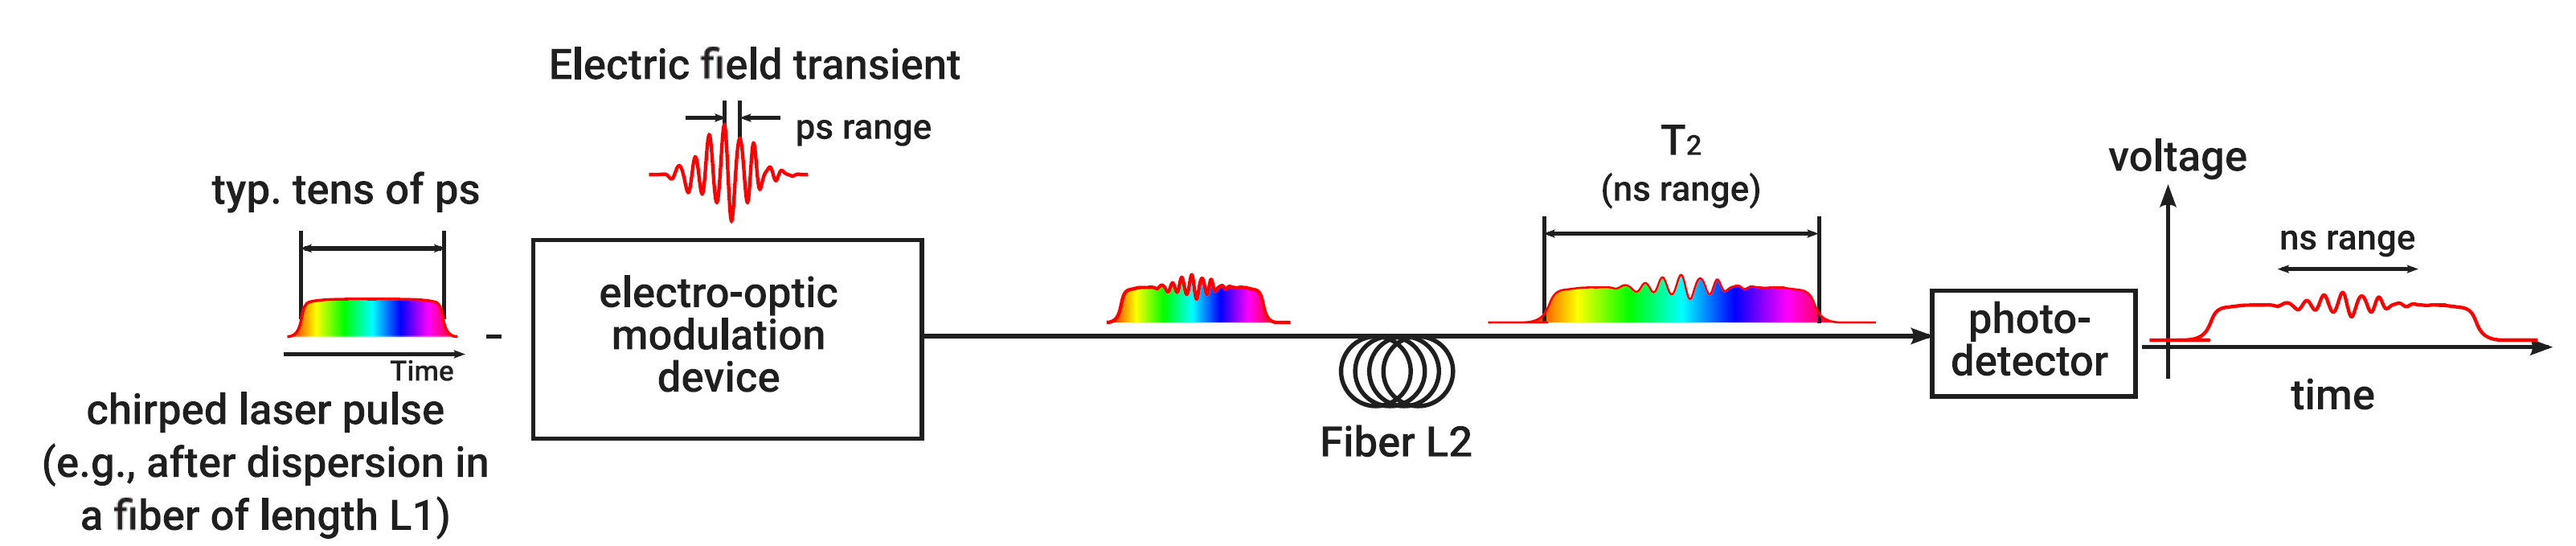
\includegraphics[width=\textwidth]{img/time_stretch}
	\end{figure}
\begin{itemize}
	\item Brief explanation of principle
\end{itemize}
\end{frame}


\section{Motivation And Objective}

\begin{frame}[t]{Motivation and Objectives}
\only<1>{
	\begin{figure}
		\centering
		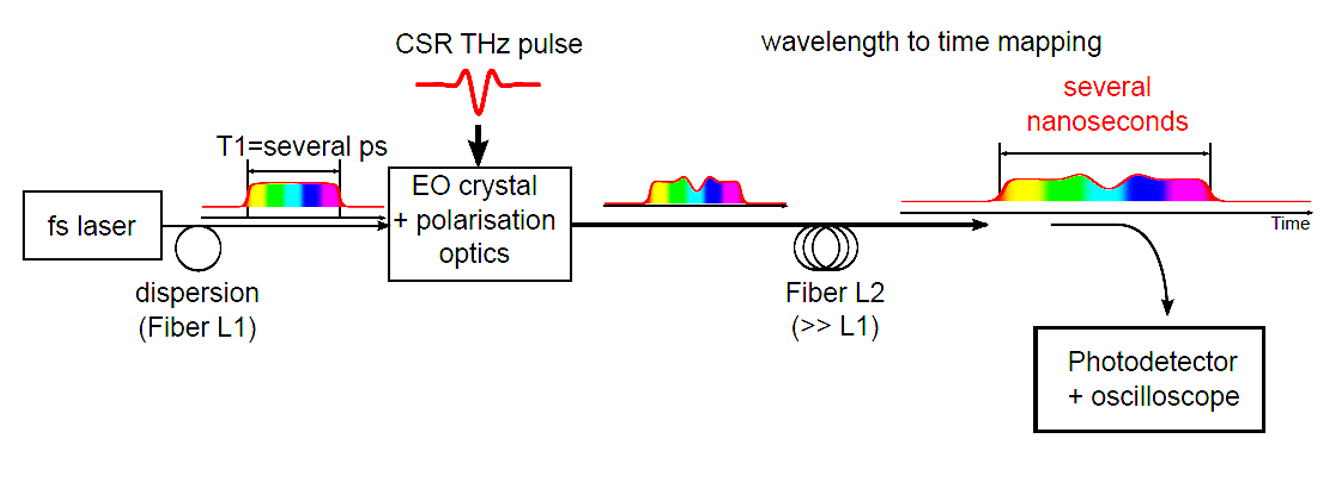
\includegraphics[width=\textwidth]{img/motivation1}
	\end{figure}	
}
\only<2>{
	\begin{figure}
		\centering
		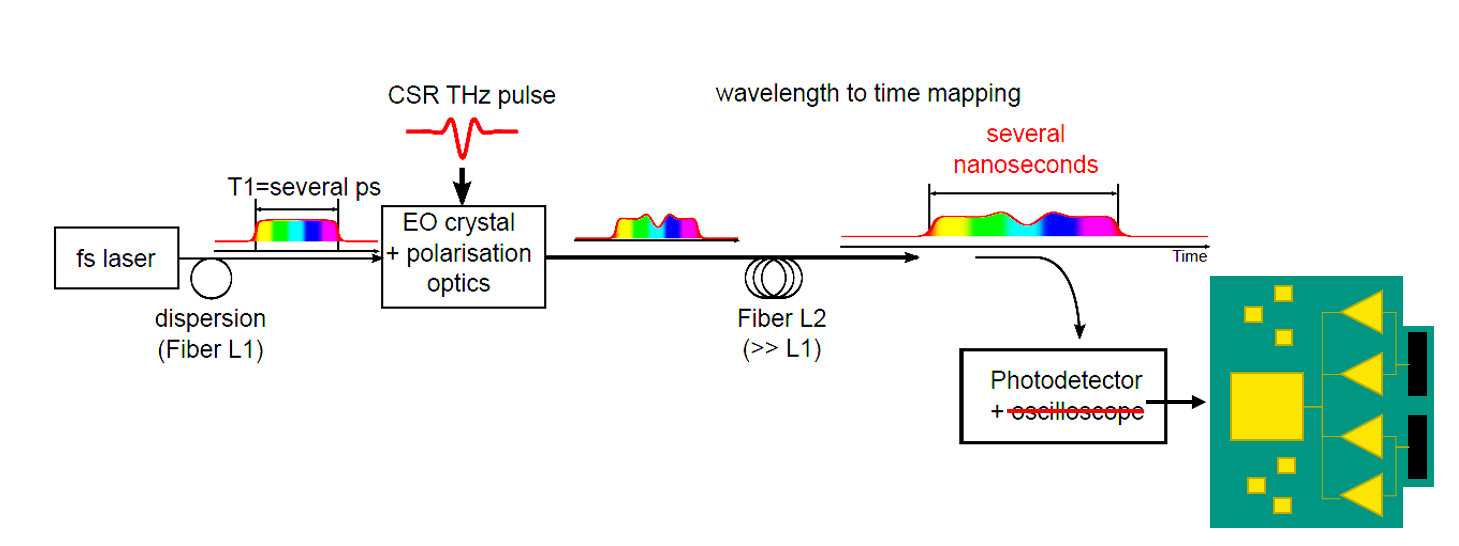
\includegraphics[width=\textwidth]{img/motivation2}
	\end{figure}
}
\only<3>{
	\begin{itemize}
		\item Optical part is done at Lille University
		\item Work @IPE: Design appropriate read-out system
	\end{itemize}
	
	\textbf{Objectives}
	\begin{itemize}
		\item Continuously sample ns pulse
		\item Using time-interleaving method for ADCs
		\item Compatibility with KARA
	\end{itemize}
}
\end{frame}


\section{Architecture}

\begin{frame}[t]{Architecture}
\only<1>{
\begin{itemize}
	\item Briefly explain KAPTURE
	\item ...
\end{itemize}	
}	
\only<2>{
	\begin{figure}
		\centering
		\resizebox{!}{0.35\linewidth}{\includegraphics[]{img/kapture.tikz}}
		\caption{KAPTURE general principle}
	\end{figure}
}
\only<3>{
	\begin{figure}
		\resizebox{!}{0.35\linewidth}{\includegraphics[]{img/detector_signal.tikz}}
		\caption{Sampled pulse}
	\end{figure}
}
\only<4>{
	\begin{figure}
		\centering
		\resizebox{!}{0.4\linewidth}{\includegraphics[]{img/theresa.tikz}}
	\end{figure}
}
\only<5>{
	\begin{figure}
		\centering
		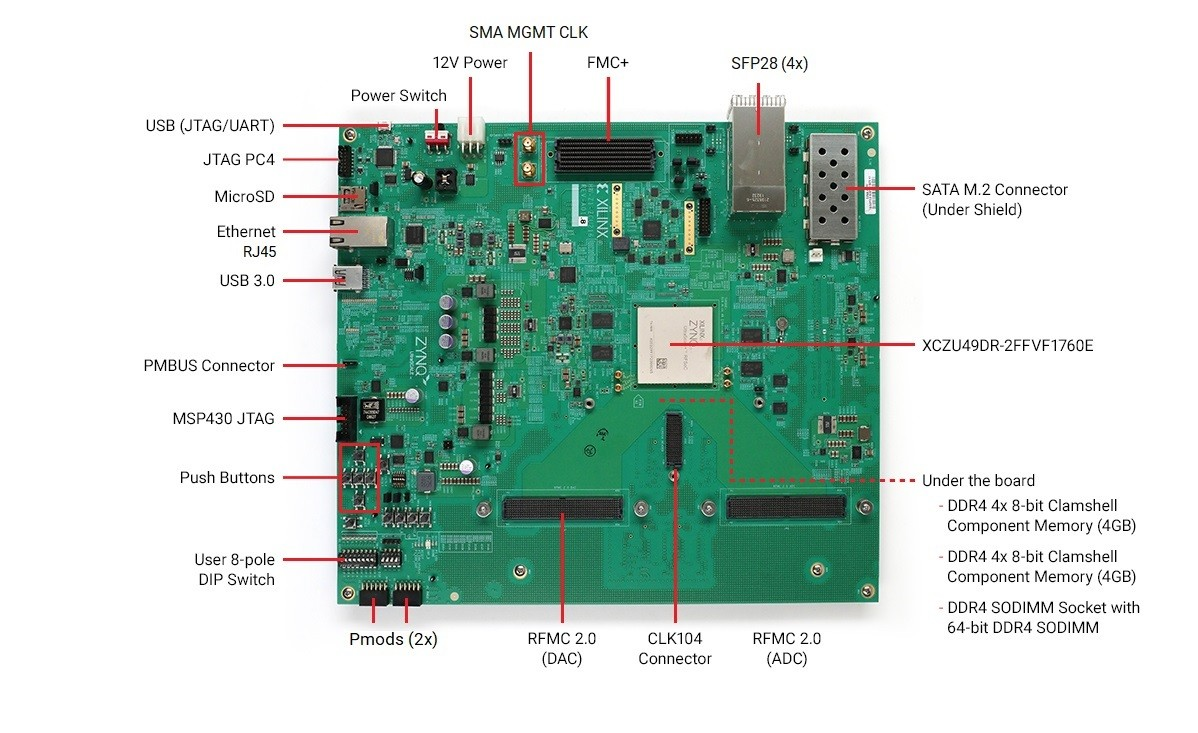
\includegraphics[width=0.7\textwidth]{img/zcu216}
	\end{figure}
}
\only<6>{
	\begin{figure}
		\centering
		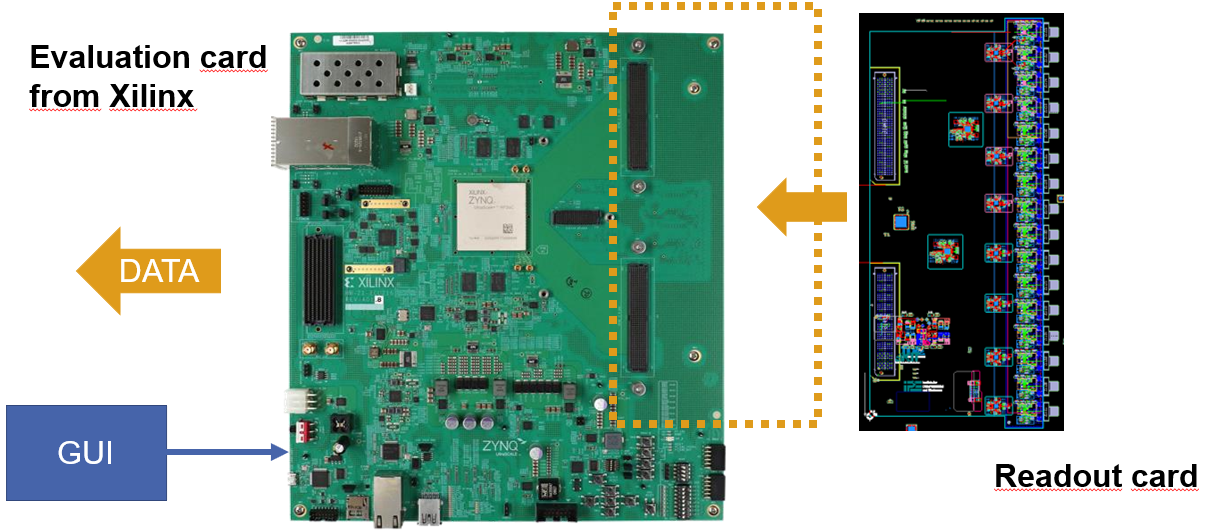
\includegraphics[width=0.7\textwidth]{img/system}
	\end{figure}
}
\end{frame}

\section{Schematics \& Layout}

\begin{frame}[t]{Schematics \& Layout}
	\begin{figure}
		\centering
		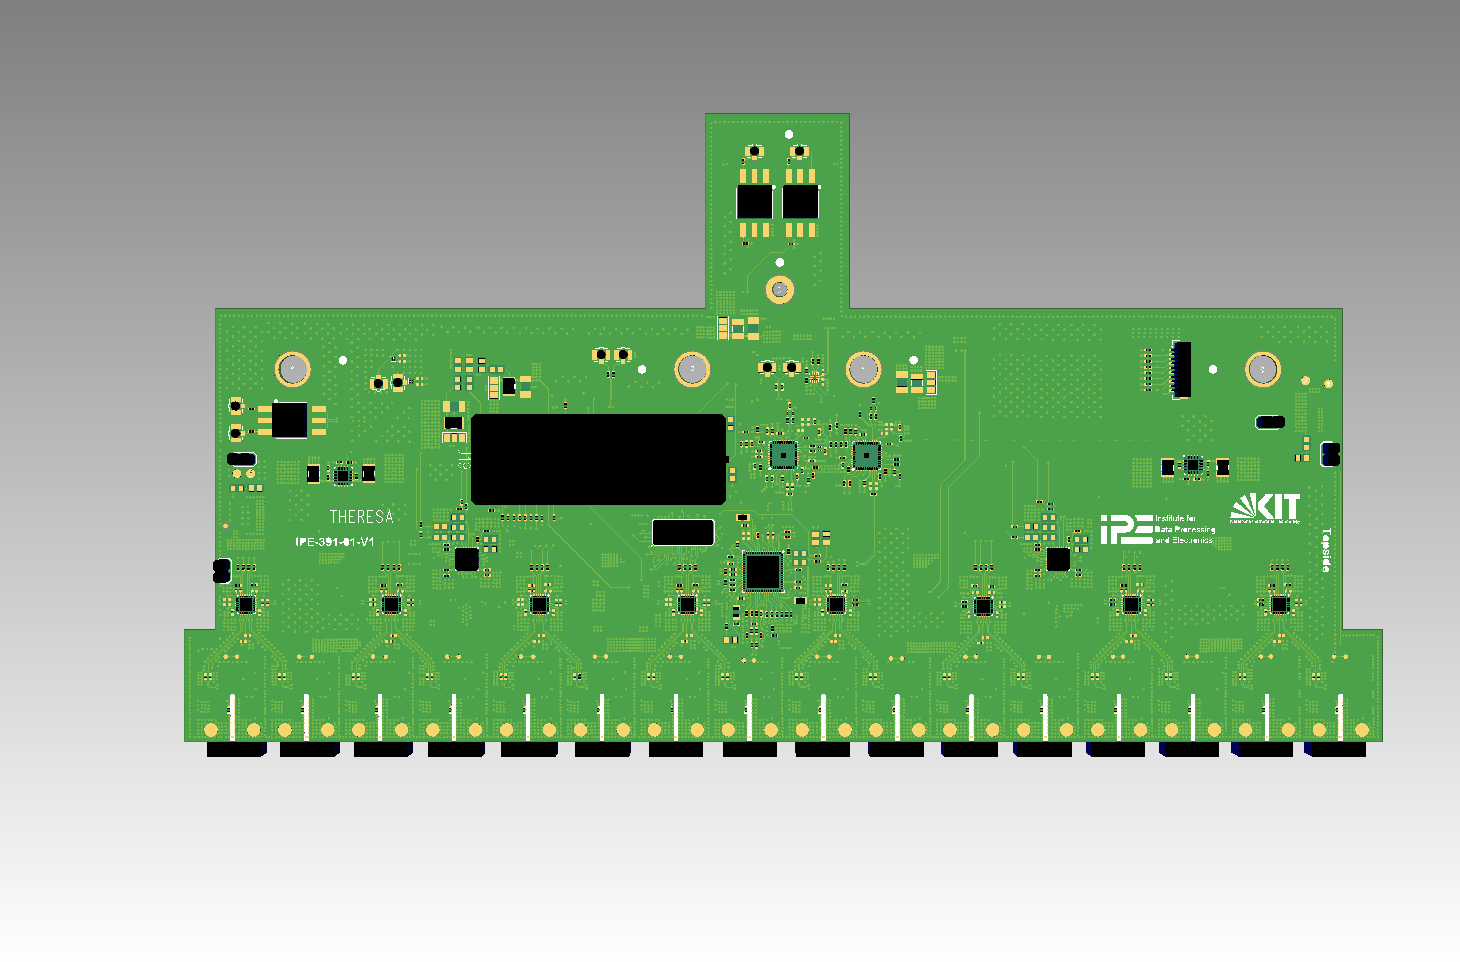
\includegraphics[width=0.6\textwidth]{img/board}
	\end{figure}
\end{frame}


%\section{Main Stuff}
%\begin{frame}[t]{A Nice Plot}
%\begin{figure}
%\centering
%\includegraphics[width=\textwidth,height=0.25\textwidth]{img/pgfplots.tikz}
%\caption{Data came to my mind when i dreamed of \cite{journals/bstj/Shannon48}}
%\end{figure}
%\begin{itemize}
%\item Tikz/PGFplot scaled with \texttt{tikzscale} in \texttt{\textbackslash includegraphics} options
%\item Using tikz library \texttt{external} to pre-compile for speed
%\end{itemize}
%\end{frame}
%
%\begin{frame}[t]{A Nice Block Diagram}
%\only<1>{
%\begin{figure}
%\centering
%\includegraphics[]{img/tikzBlockDiagram/tikzBlockDiagram1.tikz}
%\end{figure}
%}
%\only<2>{
%\begin{figure}
%\centering
%\includegraphics[]{img/tikzBlockDiagram/tikzBlockDiagram2.tikz}
%\end{figure}
%}
%\end{frame}

%\begin{frame}[t]{Next Level Circuit}
%\begin{figure}
%\centering
%\resizebox{!}{0.35\linewidth}{\includegraphics[]{img/circuit.tikz}}
%\caption{Shrink \texttt{tikzpicture} (with text and everything) to usable size}
%\end{figure}
%\end{frame}
%
%\section{Results}
%\begin{frame}[t]{The Awesome Results}
%\begin{figure}
%\centering
%\includegraphics[]{img/barplot.tikz}
%\end{figure}
%\end{frame}


%\section{Conclusion And Outlook}
%\begin{frame}[t]{Conclusion}
%\begin{itemize}
%\item The key to burning an ex-wife effigy is to dip it in paraffin wax and then toss the flaming bottle of isopropyl alcohol from a safe distance
%\item Do not stand too close when you light an ex-wife effigy
%\end{itemize}
%\only<2>{
%\begin{figure}
%\centering
%
\includegraphics[width=0.5\linewidth]{img/ron.jpg}
%\end{figure}
%}
%\end{frame}

\section{Outlook}
\begin{frame}[t]{Outlook}
\only<1>{
	\begin{itemize}
		\item Firmware: Xilinx example designs, IPE-own solutions
		\item Show picture of example design
	\end{itemize}
}
\only<2>{
	\begin{itemize}
		\item Board in production
		\item Characterization of sampling board$\rightarrow$ e.g. with Evaluation Tool
		\item Firmware development for system integration
		\item Use in experiments, e.g. KARA 
	\end{itemize}
}
\end{frame}

\appendix
\beginbackup
\begin{frame}[t]{Sources}
\printbibliography
\end{frame}

\begin{frame}[t]{Backup (1)}
\begin{itemize}
\item May help if someone asks
\end{itemize}
\end{frame}

\backupend



\end{document}